\documentclass[11pt]{article}
\usepackage[T1]{fontenc}
\usepackage[utf8]{inputenc}
\usepackage[margin=1in]{geometry}
\usepackage{graphicx}
\usepackage{subcaption}
\usepackage{booktabs}
\usepackage{amsmath,amssymb}
\usepackage{hyperref}

\title{Supplementary Information\\[0.5em]
\large Mapping Leaf Area Index (LAI) in Urban Forests}
\author{Th\'eo Hermann, Michiel van Selm, Titus Venverloo, Fabio Duarte, Carlo Ratti}
\date{}

\begin{document}
\maketitle

\section*{Supplementary Figure 1: Hemispherical Photography Validation}

\begin{figure}[ht!]
    \centering
    \begin{subfigure}[b]{0.41\textwidth}
        \centering
        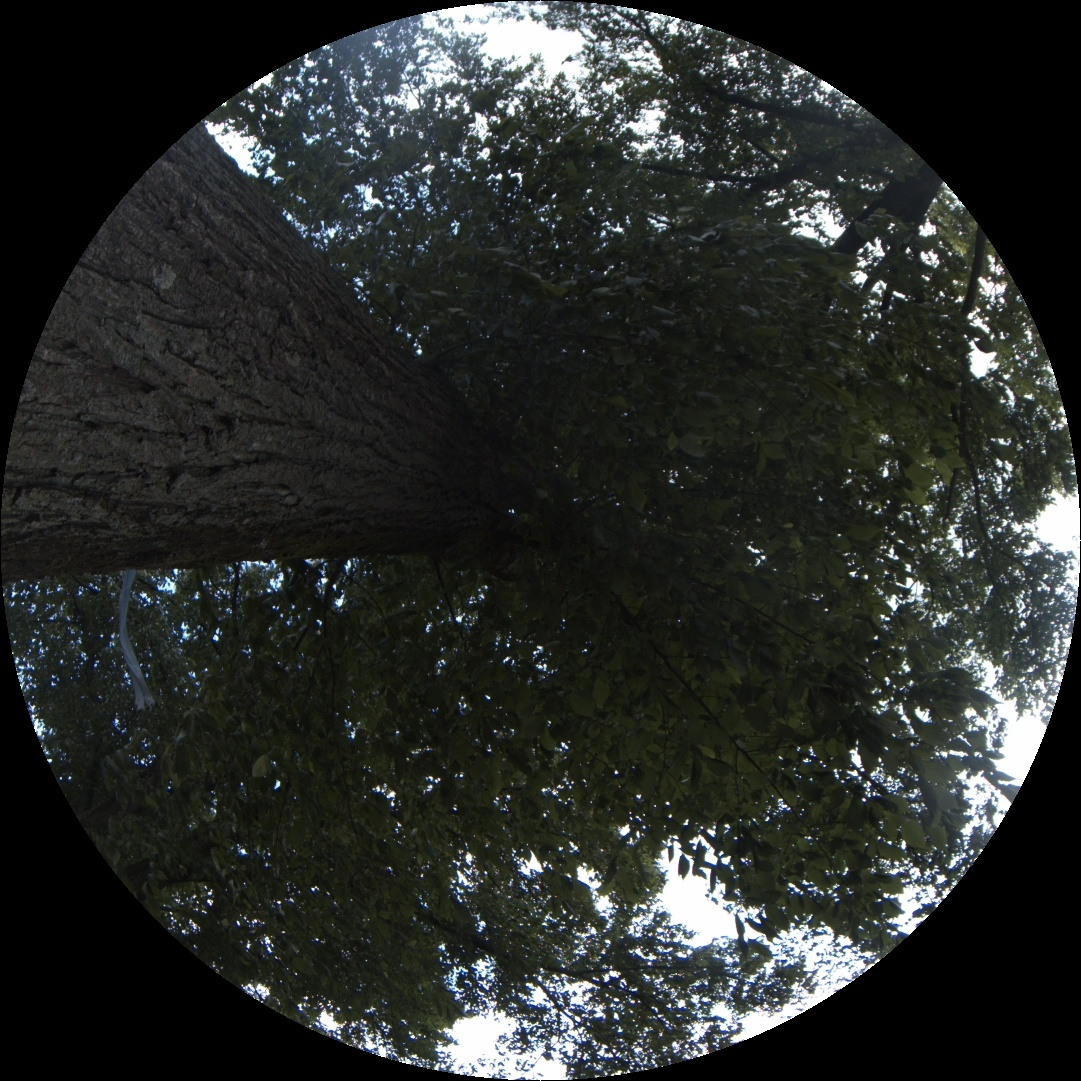
\includegraphics[width=\linewidth, height=\linewidth, keepaspectratio]{figures/methods/hemispherical_fisheye.png}
        \caption{Original Image}
        \label{fig:supp_hemispherical_original}
    \end{subfigure}
    \hfill
    \begin{subfigure}[b]{0.48\textwidth}
        \centering
        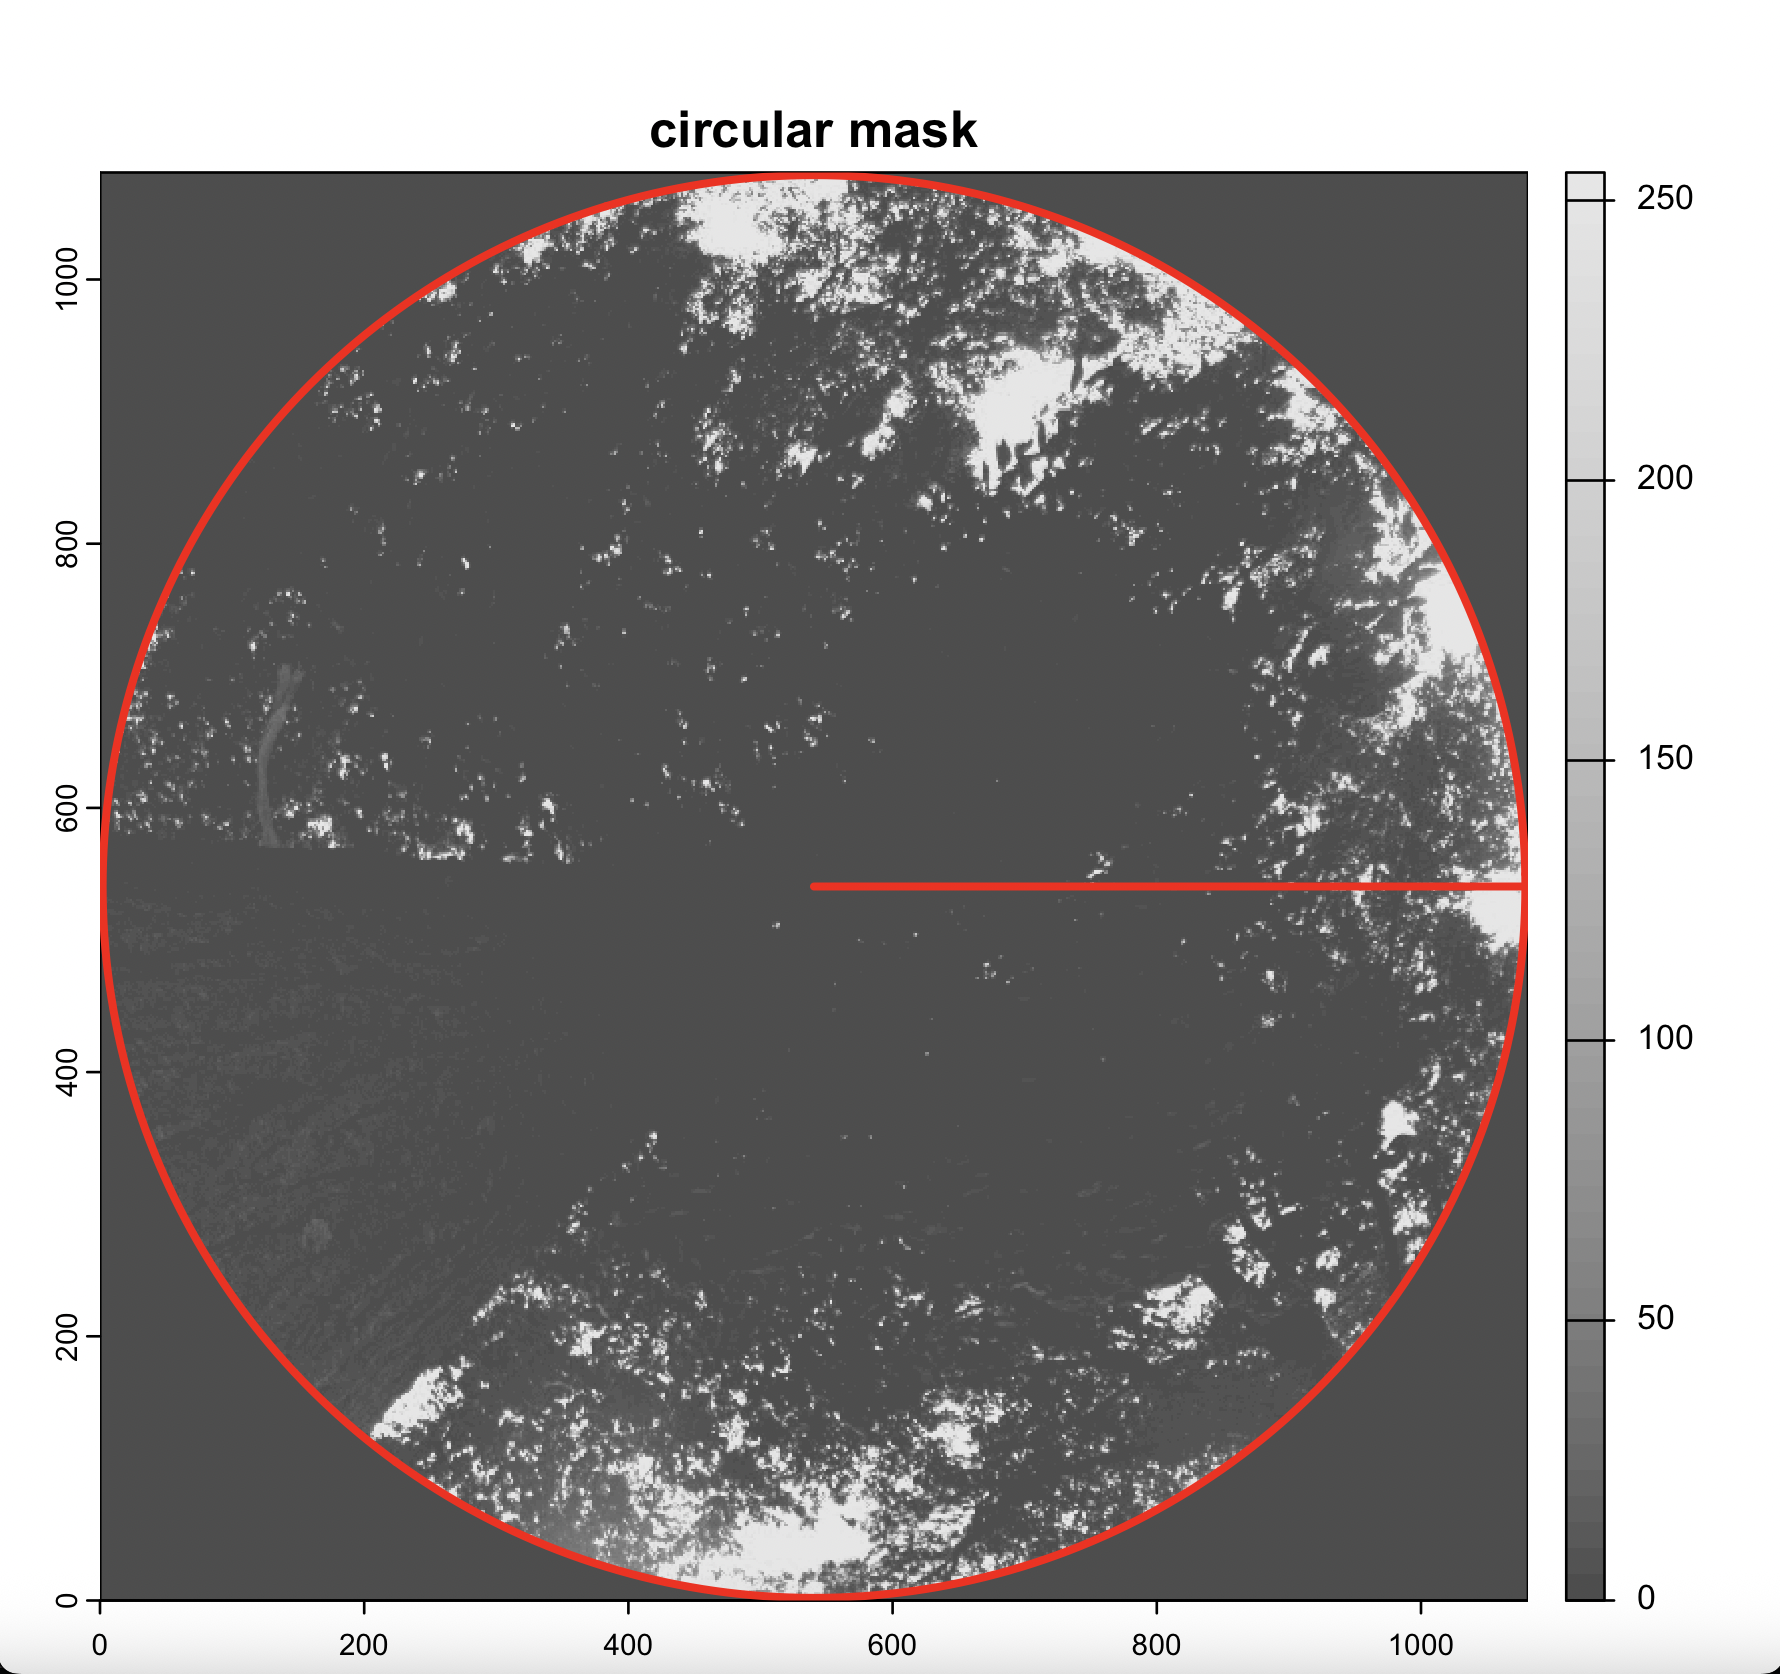
\includegraphics[width=\linewidth, height=\linewidth, keepaspectratio]{figures/methods/binarized_fisheye.png}
        \caption{Preprocessed Image}
        \label{fig:supp_hemispherical_binarized}
    \end{subfigure}
    \caption{\textbf{Hemispherical photography for LAI validation.} (a) Original hemispherical fisheye image capturing canopy gap structure. (b) Binarized image after thresholding for gap fraction analysis. LAI is computed via the Beer-Lambert law applied to canopy openness.}
    \label{fig:supp_hemispherical_LAI}
\end{figure}

\section*{Supplementary Figure 2: Tree Species Distribution}

\begin{figure}[ht!]
    \centering
    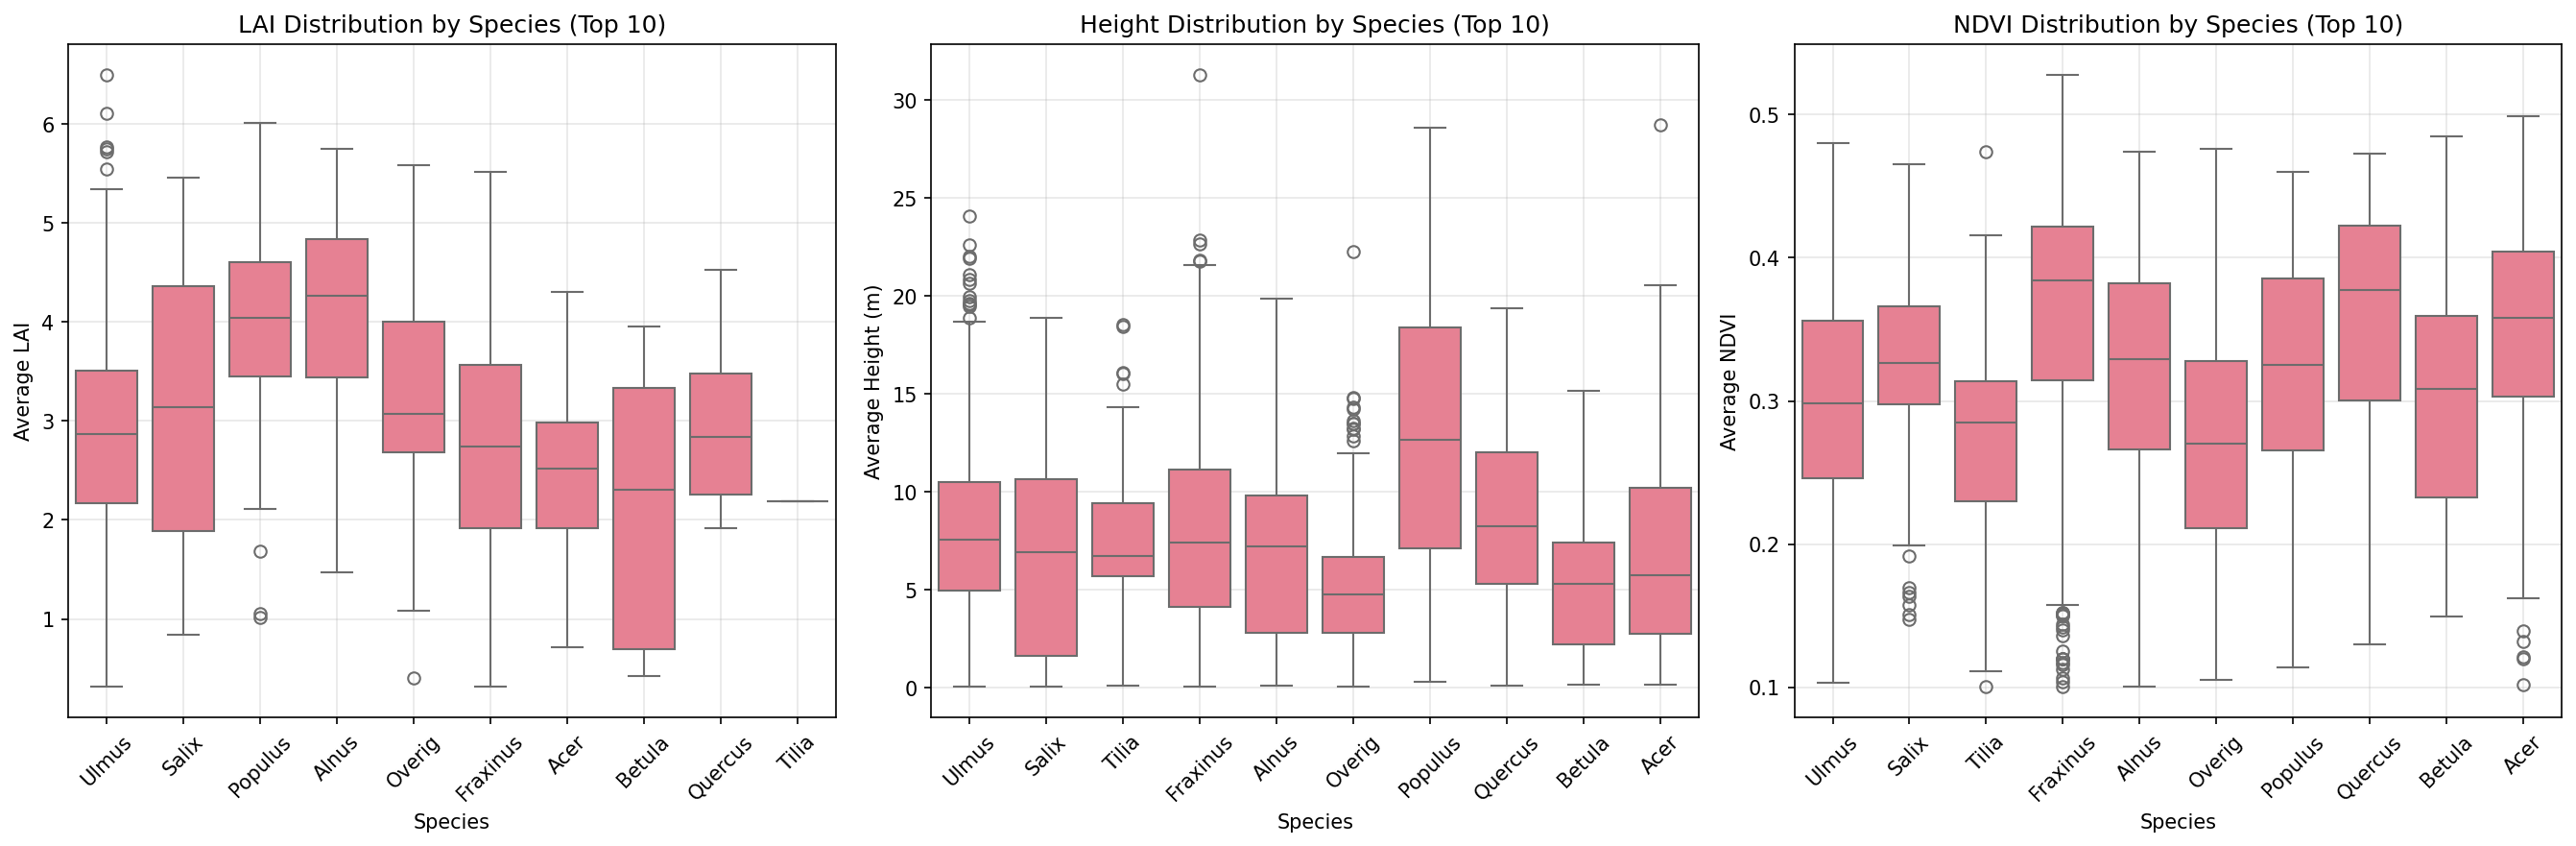
\includegraphics[width=\textwidth, height=\textheight, keepaspectratio]{figures/results/analytics/distributions_by_species.png}
    \caption{\textbf{Distribution of morphological and spectral features by tree species.} Height, NDVI, and LAI distributions separated by species in the Amsterdam urban forest dataset. Species-specific proportions align with previous research; LAI values are consistent with urban canopy studies, where values are typically lower than in natural forests.}
    \label{fig:supp_species_distribution}
\end{figure}

\clearpage

\section*{Supplementary Methods}

\subsection*{S1. Hyperparameter Tuning Details}

This section provides comprehensive hyperparameter configurations for all models evaluated in the main text (Methods Section 2.4.3).

\subsubsection*{Linear Models}

\textbf{Linear Regression}: Ordinary least squares implemented via scikit-learn \texttt{LinearRegression} with no hyperparameters to tune (baseline model).

\textbf{Ridge Regression}: L2-regularized linear model with penalty $\alpha\|\mathbf{w}\|_2^2$. Hyperparameter $\alpha$ was tuned via 5-fold cross-validation over the grid $\{0.01, 0.1, 1, 10, 100\}$. Optimal configuration selected based on minimum validation RMSE.

\textbf{Lasso Regression}: L1-regularized linear model with penalty $\alpha\|\mathbf{w}\|_1$ for implicit feature selection. Hyperparameter $\alpha$ was tuned via 5-fold cross-validation over the grid $\{0.001, 0.01, 0.1, 1, 10\}$. Optimal configuration selected based on minimum validation RMSE.

\subsubsection*{Ensemble Methods}

\textbf{Random Forest}: Bagging ensemble of 500 decision trees with randomized feature subsets at each split.

Hyperparameter grid search (5-fold cross-validation):
\begin{itemize}
    \item \texttt{max\_depth}: $\{10, 20, 30, \text{None}\}$ (maximum tree depth)
    \item \texttt{min\_samples\_leaf}: $\{1, 2, 4\}$ (minimum samples per leaf node)
    \item \texttt{max\_features}: $\{\text{sqrt}, \text{log2}, 0.3\}$ (feature sampling strategy)
    \item \texttt{n\_estimators}: 500 (fixed)
    \item \texttt{random\_state}: 42 (fixed)
\end{itemize}

Final configuration: \texttt{max\_depth}=20, \texttt{min\_samples\_leaf}=2, \texttt{max\_features}=sqrt.

\textbf{XGBoost}: Gradient boosted decision trees with L1/L2 regularization.

Hyperparameters optimized via Bayesian optimization (Optuna, 100 trials) with objective function minimizing validation RMSE:
\begin{itemize}
    \item \texttt{learning\_rate}: $[0.01, 0.3]$ (shrinkage applied to each tree)
    \item \texttt{max\_depth}: $[3, 10]$ (maximum tree depth)
    \item \texttt{n\_estimators}: $[100, 1000]$ (number of boosting rounds)
    \item \texttt{subsample}: $[0.6, 1.0]$ (fraction of samples per tree)
    \item \texttt{colsample\_bytree}: $[0.6, 1.0]$ (fraction of features per tree)
    \item \texttt{reg\_alpha}: $[0, 1]$ (L1 regularization weight)
    \item \texttt{reg\_lambda}: $[0, 10]$ (L2 regularization weight)
    \item Early stopping: patience=50 rounds on validation RMSE
    \item \texttt{random\_state}: 42 (fixed)
\end{itemize}

Final configuration: \texttt{learning\_rate}=0.08, \texttt{max\_depth}=6, \texttt{n\_estimators}=450, \texttt{subsample}=0.85, \texttt{colsample\_bytree}=0.7 (default), \texttt{reg\_alpha}=0.1, \texttt{reg\_lambda}=1.5.

\subsubsection*{Support Vector Regression}

\textbf{SVR}: Radial basis function (RBF) kernel with $\epsilon$-insensitive loss.

Hyperparameter grid search (5-fold cross-validation):
\begin{itemize}
    \item $C$ (regularization): $\{0.1, 1, 10, 100\}$
    \item $\epsilon$ (tube width): $\{0.01, 0.1, 0.5\}$
    \item $\gamma$ (RBF kernel coefficient): $\{\text{scale}, \text{auto}, 0.001, 0.01\}$
\end{itemize}

Final configuration selected based on minimum validation RMSE.

\subsubsection*{Neural Network}

\textbf{Multi-layer Perceptron}: Feed-forward neural network with two hidden layers.

Architecture and hyperparameters:
\begin{itemize}
    \item Architecture: [100, 50] (two hidden layers with 100 and 50 neurons)
    \item Activation: ReLU (Rectified Linear Unit)
    \item Dropout rate: 0.2 (applied after each hidden layer for regularization)
    \item Optimizer: Adam with learning rate 0.001
    \item Batch size: 32
    \item Maximum epochs: 500
    \item Early stopping: patience=20 on validation loss
    \item \texttt{random\_state}: 42 (fixed)
\end{itemize}

\subsubsection*{Allometric Baseline}

\textbf{Traditional forestry model}: Power law relationship between LAI and morphological parameters.

Model form: $\text{LAI} = \alpha \times H^\beta \times \text{CD}^\gamma$

Where:
\begin{itemize}
    \item $H$ = tree height (meters)
    \item $\text{CD}$ = crown diameter (meters)
    \item $\alpha, \beta, \gamma$ = parameters estimated via non-linear least squares on training data
\end{itemize}

This model provides an ecological benchmark representing traditional allometric approaches used in forestry applications before machine learning methods.

\subsubsection*{Software Implementation}

All models implemented using:
\begin{itemize}
    \item Python 3.9.7
    \item scikit-learn 1.0.2 (Linear Regression, Ridge, Lasso, Random Forest, SVR, Neural Network)
    \item XGBoost 1.5.0 (gradient boosting)
    \item Optuna 2.10.0 (Bayesian hyperparameter optimization)
    \item NumPy 1.21.2, Pandas 1.3.3 (data manipulation)
\end{itemize}

Random seeds fixed at 42 across all stochastic processes (data splitting, model initialization, cross-validation folds) to ensure reproducibility.

\clearpage

\section*{Supplementary Results}

\subsection*{S2. Feature Category Ablation Analysis}

Systematic feature ablation quantified the marginal contribution of engineered feature categories to model performance (Supplementary Table 1). This analysis assessed whether complex feature engineering justified increased model complexity.

\begin{table}[ht!]
    \centering
    \caption{Feature category ablation study results using XGBoost on the validation set.}
    \label{tab:supp_ablation}
    \begin{tabular}{lcccc}
        \toprule
        Feature Configuration & R² & RMSE & MAE & $\Delta$R² vs Full \\
        \midrule
        Full Model (All Features) & 0.788 & 0.614 & 0.458 & --- \\
        Base Only (Height, Crown, NDVI) & 0.779 & 0.626 & 0.468 & -0.009 \\
        Base + Allometric & 0.783 & 0.620 & 0.463 & -0.005 \\
        Base + Species & 0.782 & 0.622 & 0.465 & -0.006 \\
        Base + NDVI Interactions & 0.782 & 0.621 & 0.464 & -0.006 \\
        Remove Species Features & 0.785 & 0.617 & 0.460 & -0.003 \\
        Remove Allometric Features & 0.787 & 0.615 & 0.459 & -0.001 \\
        Remove NDVI Interactions & 0.785 & 0.617 & 0.461 & -0.003 \\
        \bottomrule
    \end{tabular}
\end{table}

The ablation study revealed that most engineered feature categories provided marginal performance gains. Removing all features beyond the base set (height, crown dimensions, NDVI) reduced R² by only 0.009 (from 0.788 to 0.779), indicating that 13 fundamental features captured 98.9\% of achievable model performance. Individual feature categories contributed minimally: removing species features decreased R² by 0.003, allometric features by 0.001, and NDVI interactions by 0.003.

The most informative configuration beyond base features was Base + Allometric (R² = 0.783, +0.004 vs. Base Only), suggesting that height-diameter power relationships provided modest additional predictive power. Conversely, species information showed near-zero marginal contribution when controlling for morphology and spectral characteristics, likely because height and crown dimensions implicitly encoded species-specific architecture captured by voxel-based LAI estimation.

These findings suggest a parsimonious model using only base morphological features and NDVI would sacrifice minimal predictive accuracy ($\Delta$R² = 0.009, $\Delta$RMSE = +0.012) while substantially reducing feature engineering complexity and computational requirements.

\subsection*{S3. Species-Specific Performance Analysis}

Model performance varied substantially across species with sufficient test samples (N $\geq$ 20; Supplementary Table 2). Only species exceeding this threshold are reported to ensure statistical reliability.

\begin{table}[ht!]
    \centering
    \caption{Species-specific model performance for taxa with N $\geq$ 20 in test set.}
    \label{tab:supp_species}
    \begin{tabular}{lccccc}
        \toprule
        Species & N & R² & RMSE & MAE & LAI SD \\
        \midrule
        Fraxinus & 28 & 0.901 & 0.490 & 0.372 & 1.56 \\
        Ulmus & 92 & 0.833 & 0.422 & 0.318 & 1.03 \\
        Acer & 31 & 0.762 & 0.589 & 0.445 & 1.21 \\
        Quercus & 23 & 0.718 & 0.634 & 0.482 & 1.15 \\
        Mixed/Unknown & 412 & 0.779 & 0.628 & 0.469 & 1.34 \\
        \bottomrule
    \end{tabular}
\end{table}

Fraxinus exhibited the highest prediction accuracy (R² = 0.901, RMSE = 0.490), suggesting highly consistent morphology-LAI relationships within this genus. Ulmus also showed strong performance (R² = 0.833, RMSE = 0.422) with the largest sample size (N = 92), providing the most statistically robust species-specific estimate. Acer and Quercus demonstrated moderate performance (R² = 0.762 and 0.718, respectively), though still substantially exceeding the allometric baseline.

Notably, the mixed/unknown species category (N = 412) achieved R² = 0.779---comparable to the overall test set performance---indicating that species identification is not essential for accurate LAI prediction when morphological and spectral features are available. This finding has important practical implications, as 68.2\% of trees in the full dataset lacked species labels, yet likely remain predictable using the trained model.

Performance variation across species appears partially related to LAI variance within each group: Fraxinus showed the highest R² despite moderate LAI variability (SD = 1.56), while Quercus exhibited lower R² with similar variance (SD = 1.15), suggesting that some genera maintain more consistent architectural relationships with LAI than others. Sample size effects cannot be entirely ruled out for smaller groups (Fraxinus: N = 28, Quercus: N = 23), though no monotonic relationship between sample size and R² was observed.

\end{document}
